% This file was created with tikzplotlib v0.9.14.
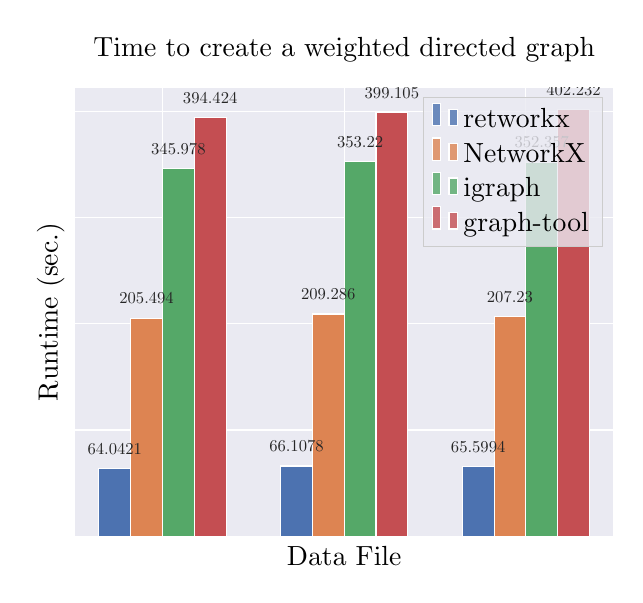
\begin{tikzpicture}

\definecolor{color0}{rgb}{0.917647058823529,0.917647058823529,0.949019607843137}
\definecolor{color1}{rgb}{0.298039215686275,0.447058823529412,0.690196078431373}
\definecolor{color2}{rgb}{0.866666666666667,0.517647058823529,0.32156862745098}
\definecolor{color3}{rgb}{0.333333333333333,0.658823529411765,0.407843137254902}
\definecolor{color4}{rgb}{0.768627450980392,0.305882352941176,0.32156862745098}

\begin{axis}[
axis background/.style={fill=color0},
axis line style={white},
legend cell align={left},
legend style={fill opacity=0.8, draw opacity=1, text opacity=1, draw=white!80!black, fill=color0},
tick align=outside,
title={Time to create a weighted directed graph},
x grid style={white},
xlabel={Data File},
xmajorgrids,
xmajorticks=false,
xmin=-0.485, xmax=2.485,
xtick style={color=white!15!black},
xtick={0,1,2},
xticklabels={USA-road-1.USA,USA-road-d.USA,USA-road-t.USA},
y grid style={white},
ylabel={Runtime (sec.)},
ymajorgrids,
ymajorticks=false,
ymin=0, ymax=422.343634314537,
ytick style={color=white!15!black}
]
\draw[draw=white,fill=color1] (axis cs:-0.35,0) rectangle (axis cs:-0.175,64.0421253204346);
\addlegendimage{ybar,ybar legend,draw=white,fill=color1}
\addlegendentry{retworkx}

\draw[draw=white,fill=color1] (axis cs:0.65,0) rectangle (axis cs:0.825,66.107777261734);
\draw[draw=white,fill=color1] (axis cs:1.65,0) rectangle (axis cs:1.825,65.5994075775147);
\draw[draw=white,fill=color2] (axis cs:-0.175,0) rectangle (axis cs:0,205.49363155365);
\addlegendimage{ybar,ybar legend,draw=white,fill=color2}
\addlegendentry{NetworkX}

\draw[draw=white,fill=color2] (axis cs:0.825,0) rectangle (axis cs:1,209.286333703995);
\draw[draw=white,fill=color2] (axis cs:1.825,0) rectangle (axis cs:2,207.229946517944);
\draw[draw=white,fill=color3] (axis cs:1.38777878078145e-17,0) rectangle (axis cs:0.175,345.978111457825);
\addlegendimage{ybar,ybar legend,draw=white,fill=color3}
\addlegendentry{igraph}

\draw[draw=white,fill=color3] (axis cs:1,0) rectangle (axis cs:1.175,353.220253801346);
\draw[draw=white,fill=color3] (axis cs:2,0) rectangle (axis cs:2.175,352.357021522522);
\draw[draw=white,fill=color4] (axis cs:0.175,0) rectangle (axis cs:0.35,394.424047040939);
\addlegendimage{ybar,ybar legend,draw=white,fill=color4}
\addlegendentry{graph-tool}

\draw[draw=white,fill=color4] (axis cs:1.175,0) rectangle (axis cs:1.35,399.104757499695);
\draw[draw=white,fill=color4] (axis cs:2.175,0) rectangle (axis cs:2.35,402.232032680511);
\draw (axis cs:-0.2625,64.0421253204346) ++(0pt,3pt) node[
  scale=0.6,
  anchor=south,
  text=white!15!black,
  rotate=0.0
]{64.0421};
\draw (axis cs:0.7375,66.107777261734) ++(0pt,3pt) node[
  scale=0.6,
  anchor=south,
  text=white!15!black,
  rotate=0.0
]{66.1078};
\draw (axis cs:1.7375,65.5994075775147) ++(0pt,3pt) node[
  scale=0.6,
  anchor=south,
  text=white!15!black,
  rotate=0.0
]{65.5994};
\draw (axis cs:-0.0875,205.49363155365) ++(0pt,3pt) node[
  scale=0.6,
  anchor=south,
  text=white!15!black,
  rotate=0.0
]{205.494};
\draw (axis cs:0.9125,209.286333703995) ++(0pt,3pt) node[
  scale=0.6,
  anchor=south,
  text=white!15!black,
  rotate=0.0
]{209.286};
\draw (axis cs:1.9125,207.229946517944) ++(0pt,3pt) node[
  scale=0.6,
  anchor=south,
  text=white!15!black,
  rotate=0.0
]{207.23};
\draw (axis cs:0.0875,345.978111457825) ++(0pt,3pt) node[
  scale=0.6,
  anchor=south,
  text=white!15!black,
  rotate=0.0
]{345.978};
\draw (axis cs:1.0875,353.220253801346) ++(0pt,3pt) node[
  scale=0.6,
  anchor=south,
  text=white!15!black,
  rotate=0.0
]{353.22};
\draw (axis cs:2.0875,352.357021522522) ++(0pt,3pt) node[
  scale=0.6,
  anchor=south,
  text=white!15!black,
  rotate=0.0
]{352.357};
\draw (axis cs:0.2625,394.424047040939) ++(0pt,3pt) node[
  scale=0.6,
  anchor=south,
  text=white!15!black,
  rotate=0.0
]{394.424};
\draw (axis cs:1.2625,399.104757499695) ++(0pt,3pt) node[
  scale=0.6,
  anchor=south,
  text=white!15!black,
  rotate=0.0
]{399.105};
\draw (axis cs:2.2625,402.232032680511) ++(0pt,3pt) node[
  scale=0.6,
  anchor=south,
  text=white!15!black,
  rotate=0.0
]{402.232};
\end{axis}

\end{tikzpicture}
